\documentstyle[11pt,graphicx]{article}
\textheight 50pc
\textwidth 41pc
\topmargin -3.0pc
\oddsidemargin 0pc
\evensidemargin -1pc
\marginparsep -1pc
\marginparwidth 0pc


\newcommand{\comment}[1]{\textit{\small {#1}}}
\newcommand{\cpp}{C\texttt{++}\ }
\newcommand{\tcl}{\textsc{Tcl\ }}
\newcommand{\ProtoMol}{\textsc{ProtoMol\ }}
\newcommand{\SamdII}{\textsc{Samd 2\ }}
\newcommand{\MOLLY}{\textsc{MOLLY\ }}

\newcommand{\tempstart}{\texttt{<}}
\newcommand{\tempend}{\texttt{>}}
\newcommand{\rij}{\mbox{r$_{ij}$}}
\newcommand{\rik}{\mbox{r$_{ik}$}}
\newcommand{\vrij}{\mbox{$\vec{r}_{ij}$}}
\newcommand{\Si}[1]{\mbox{Si$_{#1}$}}
\newcommand{\Vr}[1]{\mbox{$\vec{r}_{#1}$}}
\newcommand{\Vx}[1]{\mbox{$\vec{x}_{#1}$}}
\newcommand{\hatr}[1]{\mbox{$\hat{{r}_{#1}}$}}
\newcommand{\AbsVr}[1]{\mbox{$\left| \vec{r}_{#1} \right| $}}


\begin{document}
\title{
\begin{Large}
Proof of Angle Force Derived from Angle Energy
\end{Large}
\author{Qun Ma \& Jes\'us Izaguirre}}
\date{\today}
\maketitle

\parskip 0.3cm

%%%%%%%%%%%%%%%%%%%%%%%%%%%%%%%%%%%%%%%%%%%%%%%%%%%%%%%%%%%%%%%%%%%%%%%%%
\section{The Angle Energy and Force}
Angles describe angular bonds between three atoms. These bonds are
modeled as harmonic angular springs. The layout of three such atoms
are illustrated as in Figure~\ref{3atoms}.
\begin{figure}[hbt]
\centerline{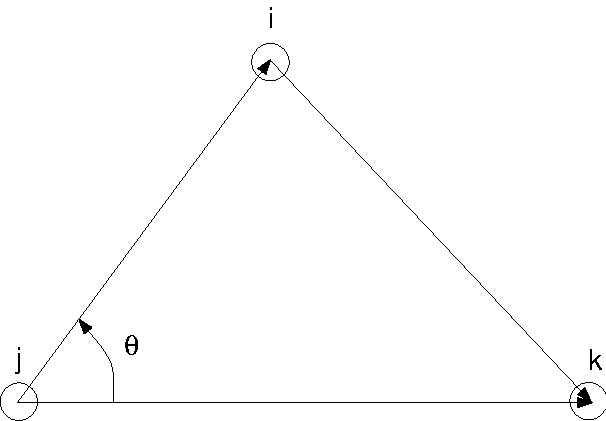
\includegraphics[width=1.5in]{3atoms.pdf}}
\caption{Layout of 3 atoms}
\label{3atoms}
\end{figure}

The energy of such a bond between atoms $i$, $j$,  and $k$ is given by:
\begin{eqnarray}
  E_{angle}  & = & E_{\theta} + E_{ub} \label{eq:AngleEnergy} \\
  E_{\theta} & = & k_{\theta} \left( \theta - \theta_0 \right)^2   \\
  E_{ub}     & = & k_{ub} \left( \AbsVr{ik} - r_{ub} \right)^2
\end{eqnarray}
\noindent
where\\
\begin{tabular}{lcl}
 $ k_{\theta} $ & =  & Force constant specified in the parameter file
for this bond type,\\ 
 $\theta $ & = &  $\cos^{-1} \left( \frac{ \Vr{ij}\, \cdot \,\Vr{kj}
}{ \AbsVr{ij} \AbsVr{kj} } \right)$, \\
$ \theta_0 $   & = & Rest angle of this bond specified in the
parameter file for this angle type,\\ 
$k_{ub}$ &=& Urey-Bradley constant, which defaults to zero, \\
  \Vr{ik}       & = & \Vr{k} - \Vr{i}, \\
  \AbsVr{ik}    & = &  $ \sqrt{(x_i - x_k)^2 + (y_i - y_k)^2 + (z_i - z_k)^2},$
                calculated distance between atoms $i$ and $k$,\\
  $ r_{ub} $    & = & Rest distance for the Urey-Bradley term.
\end{tabular}

By differentiating this formula, the force for this bond can be found to be:
\begin{equation}
\vec{F}_{angle} = - \frac{dE_{angle}}{d \vec{r}} \label{eq:angleForce}
                = \vec{F}_{\theta} + \vec{F}_{ub}
\end{equation}
where
\begin{eqnarray*}
\vec{F}_{\theta} = - \frac{dE_{\theta}}{d \theta} \cdot \frac{d
\theta}{d \vec{r} } 
                = - 2k_{\theta}(\theta - \theta_0) \cdot \frac{d
\theta}{d \vec{r} }\\ 
\vec{F}_{ub} = - \frac{dE_{ub}}{d \vec{r}} = 2 k_{ub} \left(
\AbsVr{ik} - r_{ub} \right) \hatr{ik}
\end{eqnarray*}
where $\hatr{ik}$ is the unit vector in the direction of $\vec{r_{ik}}.$
Hence the angle force on atoms $i$, $j$, and $k$ is calculated as:
\begin{eqnarray}
\label{force_i}
   F_{\vec{r}}^i & = &\left( \frac{ 2k_{\theta}(\theta - \theta_0) }{
\sin(\theta) \AbsVr{ij} } \right)  
             \left( \frac{ \vec{r_{ij}} \, \cos(\theta) }{ \AbsVr{ij}
} - \frac{\vec{r_{kj}}}{\AbsVr{kj} } \right) 
             + 2 k_{ub} \left( \AbsVr{ik} - r_{ub} \right)
\frac{\vec{r_{ik}}}{\AbsVr{ik}} \\
\label{force_k}
   F_{\vec{r}}^k & = & \left( \frac{ 2k_{\theta}(\theta - \theta_0) }{
\sin(\theta) \AbsVr{kj} } \right)  
             \left( \frac{ \vec{r_{kj}} \, \cos(\theta) }{ \AbsVr{kj}
} - \frac{\vec{r_{ij}}}{\AbsVr{ij} } \right) 
             + 2 k_{ub} \left( \AbsVr{ik} - r_{ub} \right)
\frac{\vec{r_{ki}}}{\AbsVr{ki}}\\
\label{force_j}
   F_{\vec{r}}^j & = & - \left( F_{\vec{r}}^i + F_{\vec{r}}^k \right). 
\end{eqnarray}

\section{The Proof of the Force Expression}
The proof of the force expression follows a straight-forward approach
-- application of ``chain rule.'' Let 
\begin{equation}
C(\alpha, \beta, \gamma)=\frac{\alpha + \beta - \gamma}{2
\sqrt{\alpha}\sqrt{\beta}} 
\end{equation}
where $\alpha$, $\beta$ and $\gamma$ are scalars, and $\alpha =
\AbsVr{ij}^2$, $\beta = \AbsVr{kj}^2$, $\gamma = \AbsVr{ki}^2$. It 
then follows that the angle energy can be expressed as follows
\begin{equation}
E_{\theta}(C(\alpha, \beta, \gamma)) = k_{\theta} (\theta - \theta_{0})^2
\end{equation}
where
$\theta = \cos^{-1}(C(\alpha, \beta, \gamma))$ since $\frac{ \Vr{ij}\,
\cdot \,\Vr{kj}}{ \AbsVr{ij} \AbsVr{kj}} = C(\alpha, \beta, \gamma). $
The force (negative gradient of the energy) is derived as follows.
\begin{equation}
F_{\theta} = - 
\bigtriangledown_{\vec{r}}E_{\theta} = - E_{C} \,\,C_r
\end{equation}
where 
\begin{eqnarray}
E_{C}&\equiv& \frac{dE_{\theta}}{dC} 
= - \frac{2 k_{\theta} (\theta - \theta_0)}{\sqrt{1-C^2}} 
= - \frac{2 k_{\theta} (\theta - \theta_0)}{\sin\theta} \\
C_r  &\equiv& 
\bigtriangledown_{\vec{r}} C = f \, \alpha_r + 
g \, \beta_r + 
h \, \gamma_r
\end{eqnarray}
where
\begin{eqnarray}
f &\equiv& \frac{\partial C}{\partial \alpha} =
\frac{\alpha - \beta + \gamma} 
{4\,\alpha^{3/2}\sqrt{\beta}} \\
g &\equiv& \frac{\partial C}{\partial \beta} = 
\frac{-\alpha + \beta + \gamma}
{4\,\sqrt{\alpha}\, \beta^{3/2}} \\
h &\equiv& \frac{\partial C}{\partial \gamma} 
= -\frac{1}{2\, \sqrt{\alpha}\, \sqrt{\beta}} \\
\alpha_{r} &\equiv&  \frac{d\alpha}{d\vec{r}} = (-2, 2, 0)
\sqrt{\alpha} \,\,\hatr{ij} \\
 \beta_{r} &\equiv& \frac{d\beta}{d\vec{r}} = (0, 2, -2) 
\sqrt{\beta} \,\,\hatr{kj}\\
\gamma_{r} &\equiv& \frac{d\gamma}{d\vec{r}} = (2, 0, -2) 
\sqrt{\gamma} \,\,\hatr{ki}.
\end{eqnarray}

The differention of a scalar variable w.r.t. a vector follows a
standard procedure.
\footnote{
$\vec{r} = (\Vr{i},\Vr{j},\Vr{k})$ and in the next few sections, $r 
\equiv \vec{r}.$
$\alpha_{r} \equiv \frac{d\alpha}{d\vec{r}} =
(\frac{\partial\alpha}{\partial\Vr{i}},\frac{\partial\alpha}{\partial\Vr{j}},\frac{\partial\alpha}{\partial\Vr{k}}) $
where 
$\frac{\partial\alpha}{\partial\Vr{i}} = -2 \sqrt{\alpha} \hatr{ij},$
$\frac{\partial\alpha}{\partial\Vr{j}} =  2 \sqrt{\alpha} \hatr{ij},$
and $\frac{\partial\alpha}{\partial\Vr{k}} = 0.$}


It follows that the force acted on atom $i$ is expressed as
\begin{equation}
F_{\theta}^{i} = - E_C\,(-2 \sqrt{\alpha} \hatr{ij} \, f +
2 \sqrt{\gamma} \hatr{ki} \, h) 
\end{equation}
Because $\sqrt{\gamma} \, \hatr{ki} = \vec{r_{kj}}\,- \, \vec{r_{ij}}$ 
and $\sqrt{\alpha} \, \hatr{ij} = \vec{r_{ij}},$
one has
\begin{eqnarray}
F_{\theta}^{i} &=& \frac{2 k_{\theta} (\theta - \theta_0)}{\sin\theta}\,
(-2 \vec{r_{ij}} \, f +
2 (\vec{r_{kj}}\,- \, \vec{r_{ij}}) \, h)\nonumber \\
&=&  \frac{2 k_{\theta} (\theta - \theta_0)}{\sin\theta}\,
(-2 \vec{r_{ij}}\, \frac{\alpha - \beta + \gamma} 
{4\,\alpha^{3/2}\sqrt{\beta}} +
(\vec{r_{kj}}\,- \, \vec{r_{ij}}) (-\frac{1}{\sqrt{\alpha}\,
\sqrt{\beta}})) \nonumber \\
&=&  \frac{2 k_{\theta} (\theta - \theta_0)}{\sin\theta}\,
(- \frac{\alpha - \beta + \gamma} 
{2\,\alpha^{3/2}\sqrt{\beta}}\,\vec{r_{ij}} +
\frac{1}{\sqrt{\alpha}\,
\sqrt{\beta}}  \vec{r_{ij}} \,-\,\frac{1}{\sqrt{\alpha}\,
\sqrt{\beta}}  \vec{r_{kj}})\nonumber \\
&=&  \frac{2 k_{\theta} (\theta - \theta_0)}{\sin\theta}\,
(\frac{\alpha + \beta - \gamma} 
{2\,\alpha^{3/2}\sqrt{\beta}}\,\vec{r_{ij}} \,-\,\frac{1}{\sqrt{\alpha}\,
\sqrt{\beta}}  \vec{r_{kj}})\nonumber \\
&=&  \frac{2 k_{\theta} (\theta - \theta_0)}{\sin\theta}\,
(\frac{1}{\alpha} \frac{\alpha + \beta - \gamma} 
{2\,\sqrt{\alpha} \sqrt{\beta}}\,\vec{r_{ij}} \,-\,\frac{1}{\sqrt{\alpha}\,
\sqrt{\beta}}  \vec{r_{kj}})\nonumber \\
& = & \left(\frac{ 2k_{\theta}(\theta - \theta_0) }{ \sin(\theta) \AbsVr{ij}
} \right) \left( \frac{ \vec{r_{ij}} \, \cos(\theta) }{ \AbsVr{ij} } -
\frac{\vec{r_{kj}}}{\AbsVr{kj} } \right).
\end{eqnarray}

The Urey-Bradley force acted on atom $i$ is as follows.
\begin{equation}
\vec{F}_{ub}^i = 2 k_{ub} \left(
\AbsVr{ik} - r_{ub} \right) \frac{\vec{r_{ik}}}{\AbsVr{ik}}.
\end{equation}

The total force is the summation of the two terms. It is seen that the
force on atom $i$ is same as given in Equation~{\ref{force_i}}. One
can use the symetry of atoms $i$ and $k$ to verify the correctness of 
Equation~{\ref{force_k}}. The correctness of Equation~{\ref{force_j}}
can be verified using the second law of force by Newton, ``The force
acted on object i by object j is same as that acted on object j by
object i in magnitude but in the opposite direction.'' End of proof.


\end{document}



